\chapter{Introduction}

Image processing has been a very important research domain the last years, the ever increasing number of images present on the Internet becoming more and more challenging to index, store and analyze.\\
Privacy and copyright have also been big issues which have been discussed and assessed for a long time, major users in the photography industry wanting to know at all times when someone is using or modifying one of their photos.

\section{Requirements}

We want to design a scalable algorithm which can maintain a large set of images, and perform queries of finding a highly similar image with a given input one. \\
The algorithm should be focused on copyright detection, so it should be able to determine if the input image is one of the images in the dataset, with possible transformations applied upon it:
\begin{itemize}
	\item watermarks
	\item scaling
	\item cropping
	\item various filters
\end{itemize}

As said above, the granularity of the algorithm should be able to distinguish between two lightly similar images (e.g. two different pictures of the Eiffel Tower, made by two different persons) and two images, one of which is obtained from the other.\\

The running time of the algorithm is also a major factor which should be seriously taken into consideration. It should be able to handle a large number of queries and provide a small response-time per query. Of course, there is a close connection between the running time of the algorithm and its precision, connection which should be closely analyzed in order to create a balance between the two.

In Figure~\ref{fig:basicUsage}, we can see an example usage of the algorithm. The large database is queried with the image in the bottom-left corner, and the algorithm is capable is returning the original image (even if the query image has been cropped, rotated and a gray filtered applied).

\begin{figure}[ht!]
\centering
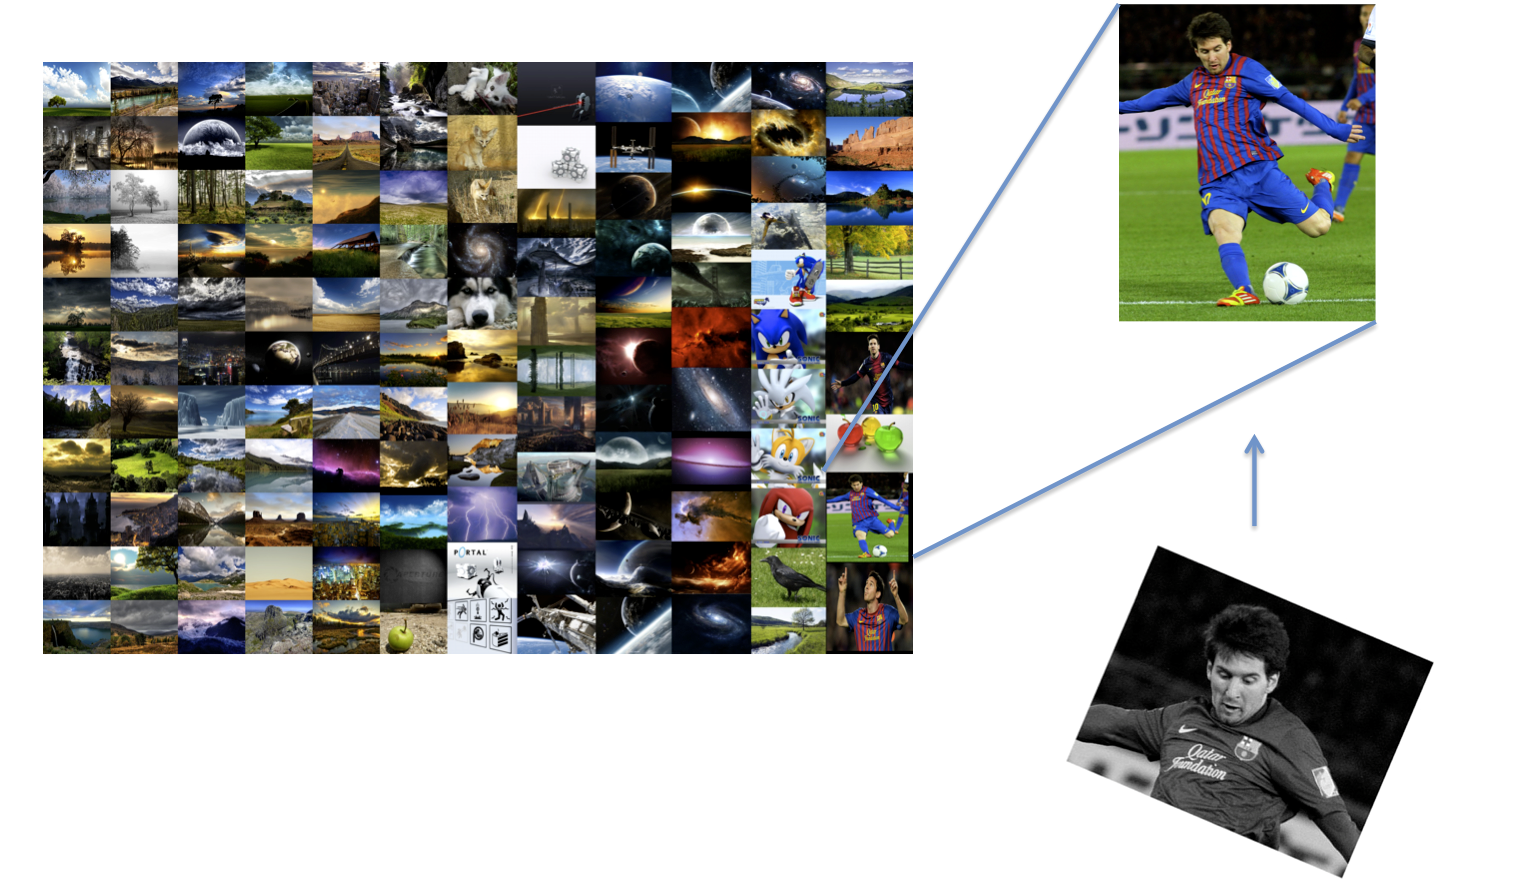
\includegraphics[width=.8\linewidth]{images/basicUsage.png}
\caption{Basic usage of our algorithm}
\label{fig:basicUsage}
\end{figure}